%\section{Réalisation et gestion du projet}

\section{Description des entrées sorties}

Dans ce projet nous avons rencontré trois termes principaux: T2M, M2M,
M2T.

La transformation text-à-modèle est la première partie dans laquelle
on reçoit en entrée un fichier \texttt{.yml}. Il a la syntaxe normal
de \texttt{YAML} avec respect des régles définit en méta-modèle créé
auparavant. Cela se manifeste par l'utilisation des mots-clés définit
en \texttt{xtext} et inspirée du méta-modèles.

\begin{figure}[H]
  \begin{center}
      \fbox{
      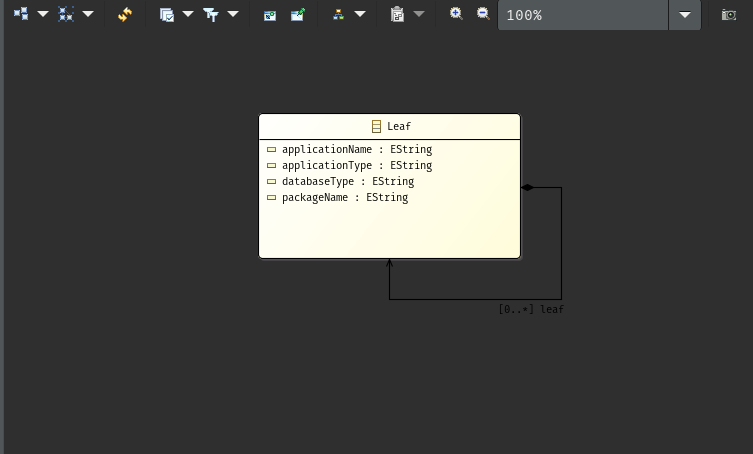
\includegraphics[width=16cm]{mmyml.png}
      }
      \caption{Les entrées de la transformation T2M}
  \end{center}
\end{figure}

L'étape qui suit est la transformation M2M. Cella, se fait en se
basant sur le modèle généré aprés la tranformation T2M. les deux
modèles générée sont des fichiers \texttt{XML}. L'outil de la
transformation utilisé est \texttt{ATL}. À la base du fichier
\texttt{main.atl}, où on a définit les régles de la transformation, on
génére le modèle \texttt{JDL}.

\begin{figure}[H]
  \begin{center}
      \fbox{
      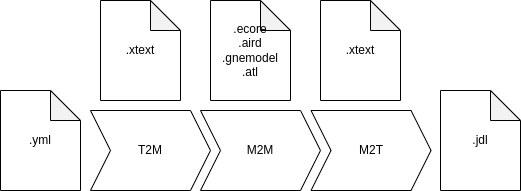
\includegraphics[width=16cm]{demarche.png}
      }
      \caption{La transformation M2M}
  \end{center}
\end{figure}

Enfin, on arrive à effectuer un tranformation \texttt{M2T} en
utilisant \texttt{xtext} une autre fois. Ceci permet de générer un
fichier \texttt{.jdl}, réspectant la syntaxe de \texttt{JDL}.

\begin{figure}[H]
  \begin{center}
      \fbox{
      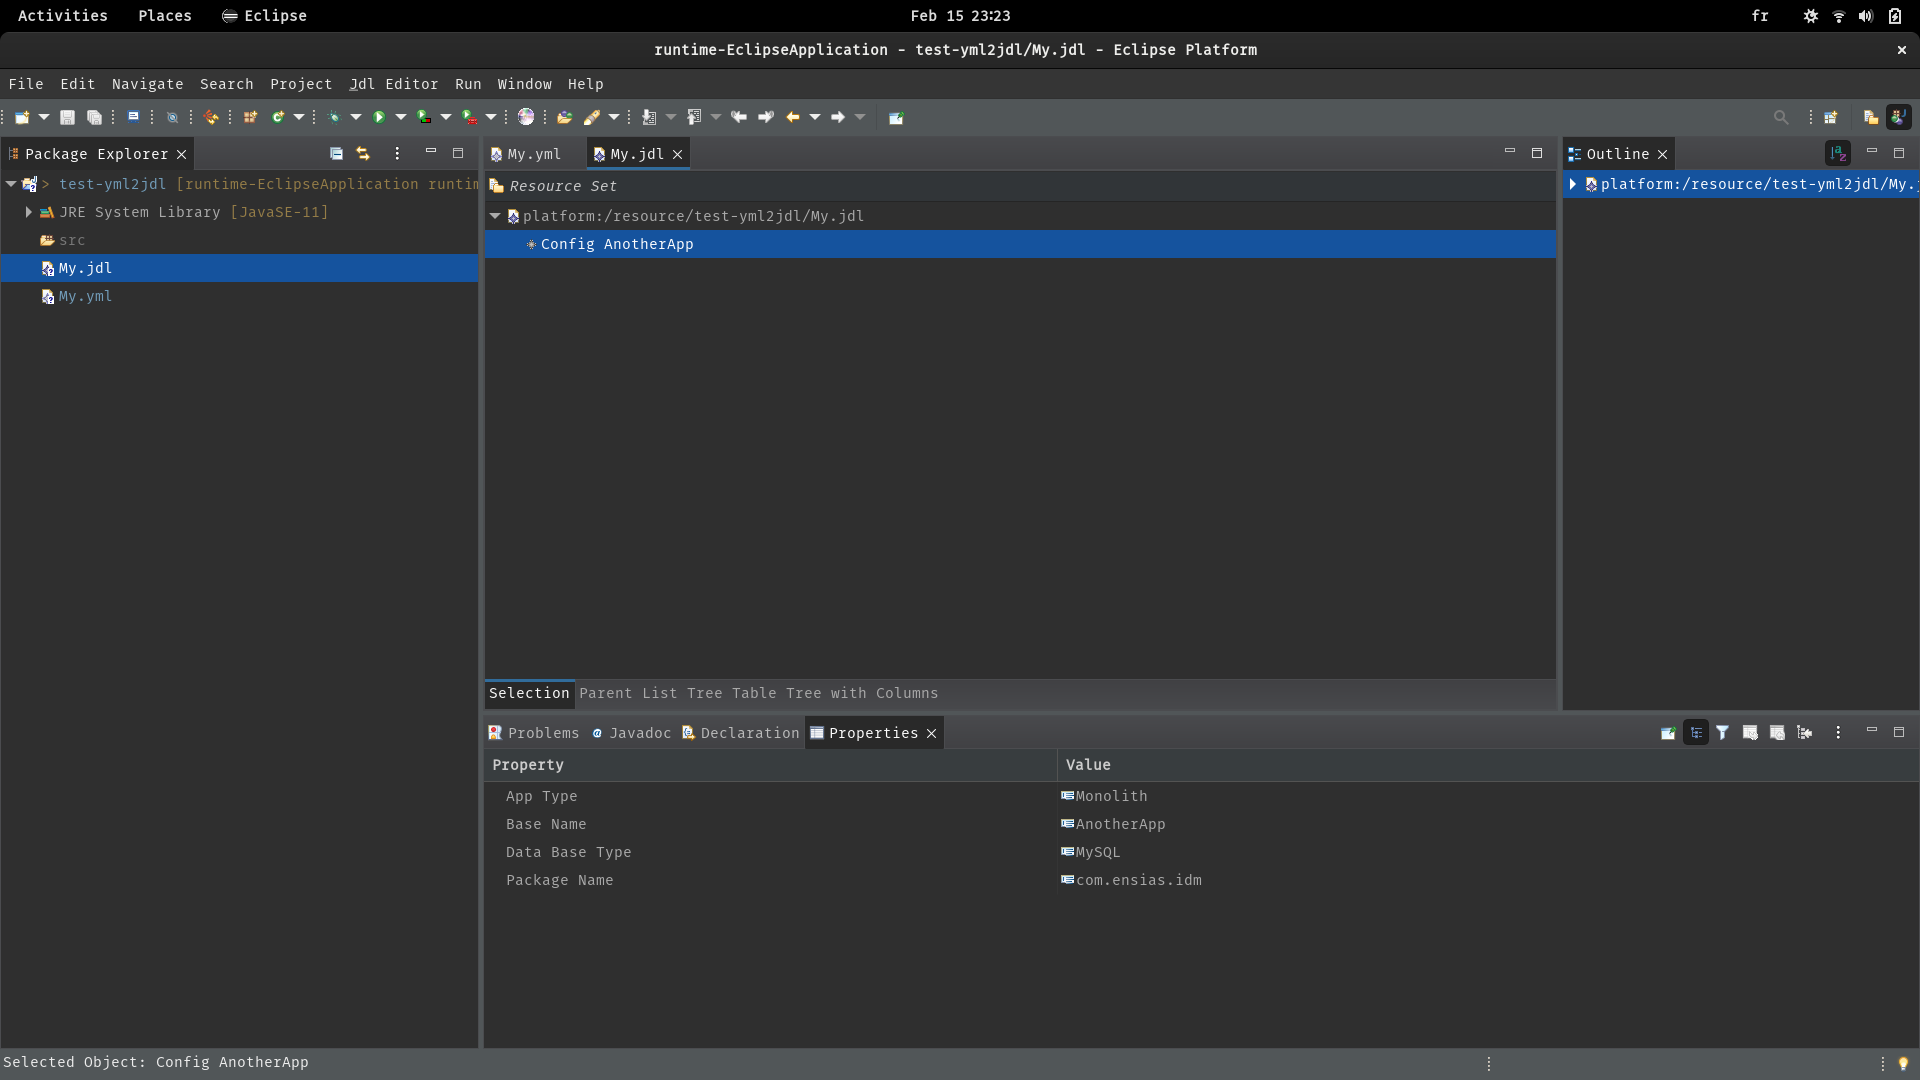
\includegraphics[width=16cm]{myjdl.png}
      }
      \caption{Les sorties de la transformation M2T}
  \end{center}
\end{figure}

\section{Mode de travail}

Il est primordial de bien gérer chaque projet et d'avoir une structure
claire et optimisée à suivre. Du coût, nous avons utiliser les outils
offers par la platforme Github pour la gestion de ce projet:

Chaque tâche est représenté par un "issue", quoi doit être assigné
manuallement à un memebre d'équipe:

\begin{figure}[H]
  \begin{center}
      \fbox{
      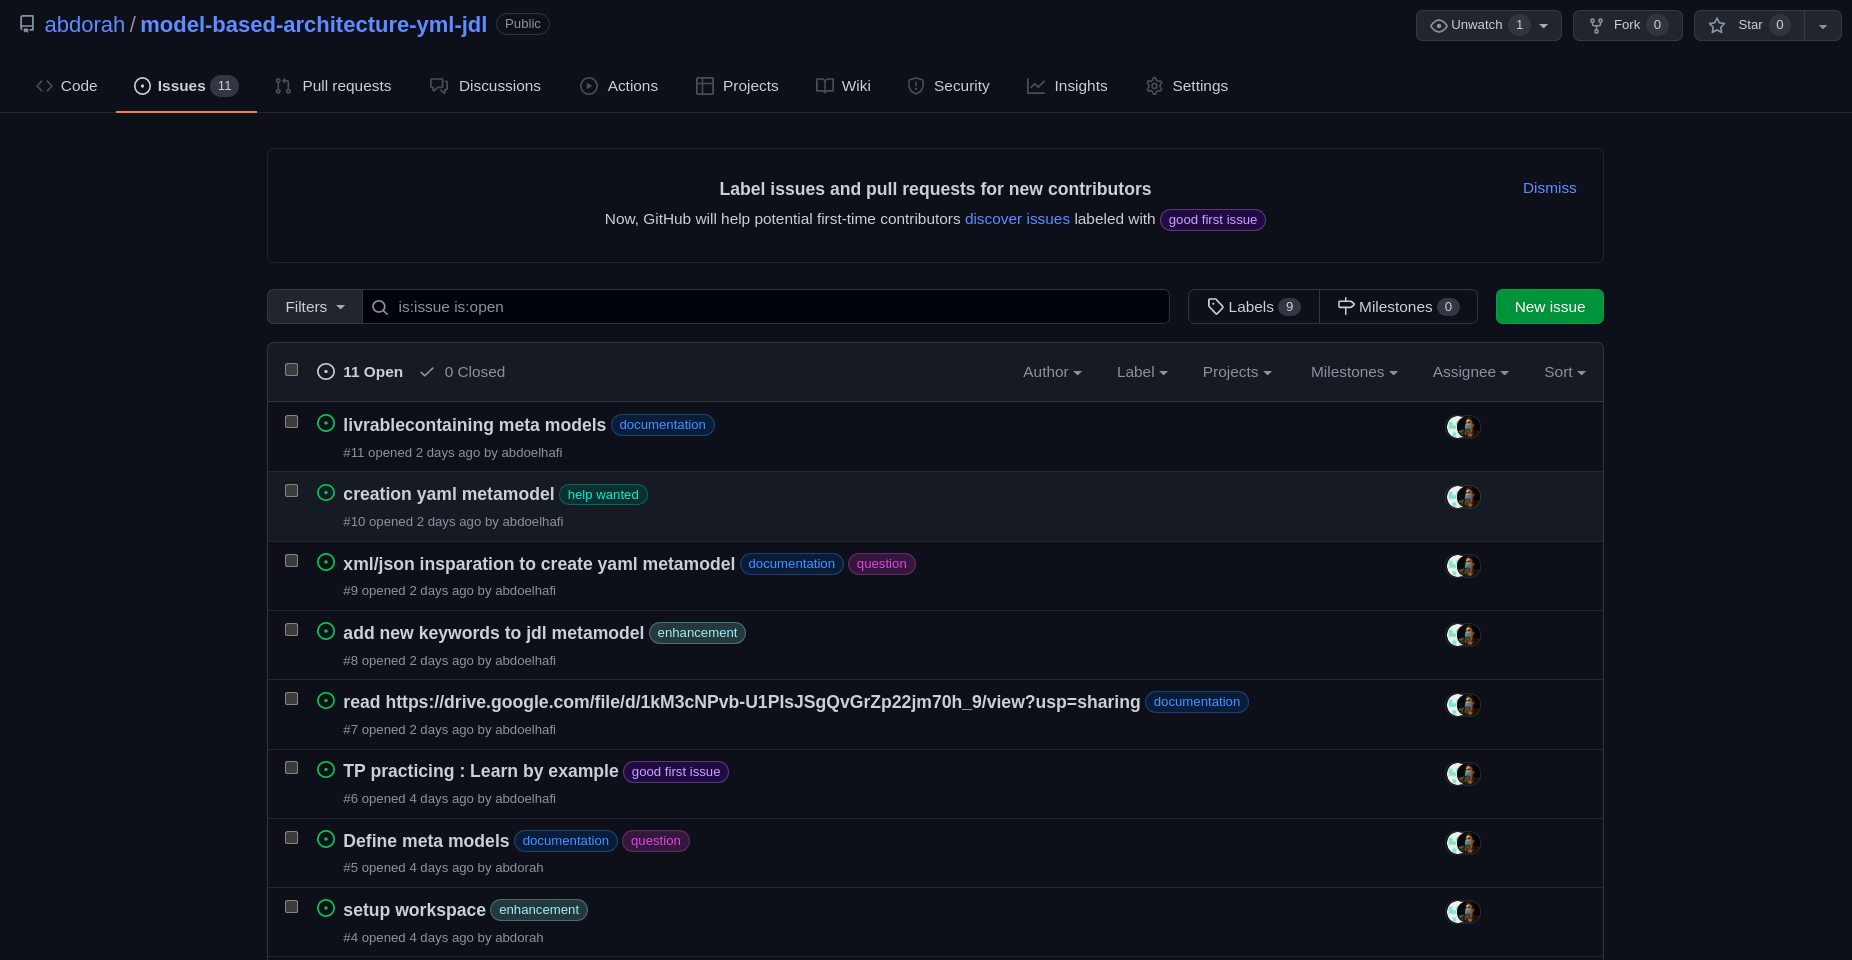
\includegraphics[width=16cm]{issues.png}
      }
      \caption{Liste des issues en Github}
  \end{center}
\end{figure}

Chaque issue est représenté par un ticket sur un tableau ayant la même
structure comme les tableux trello. Il contient touts les informations
necessaire sur le type, la définition, et l'état d'issue qu'en
concerne:

\begin{figure}[H]
  \begin{center}
      \fbox{
      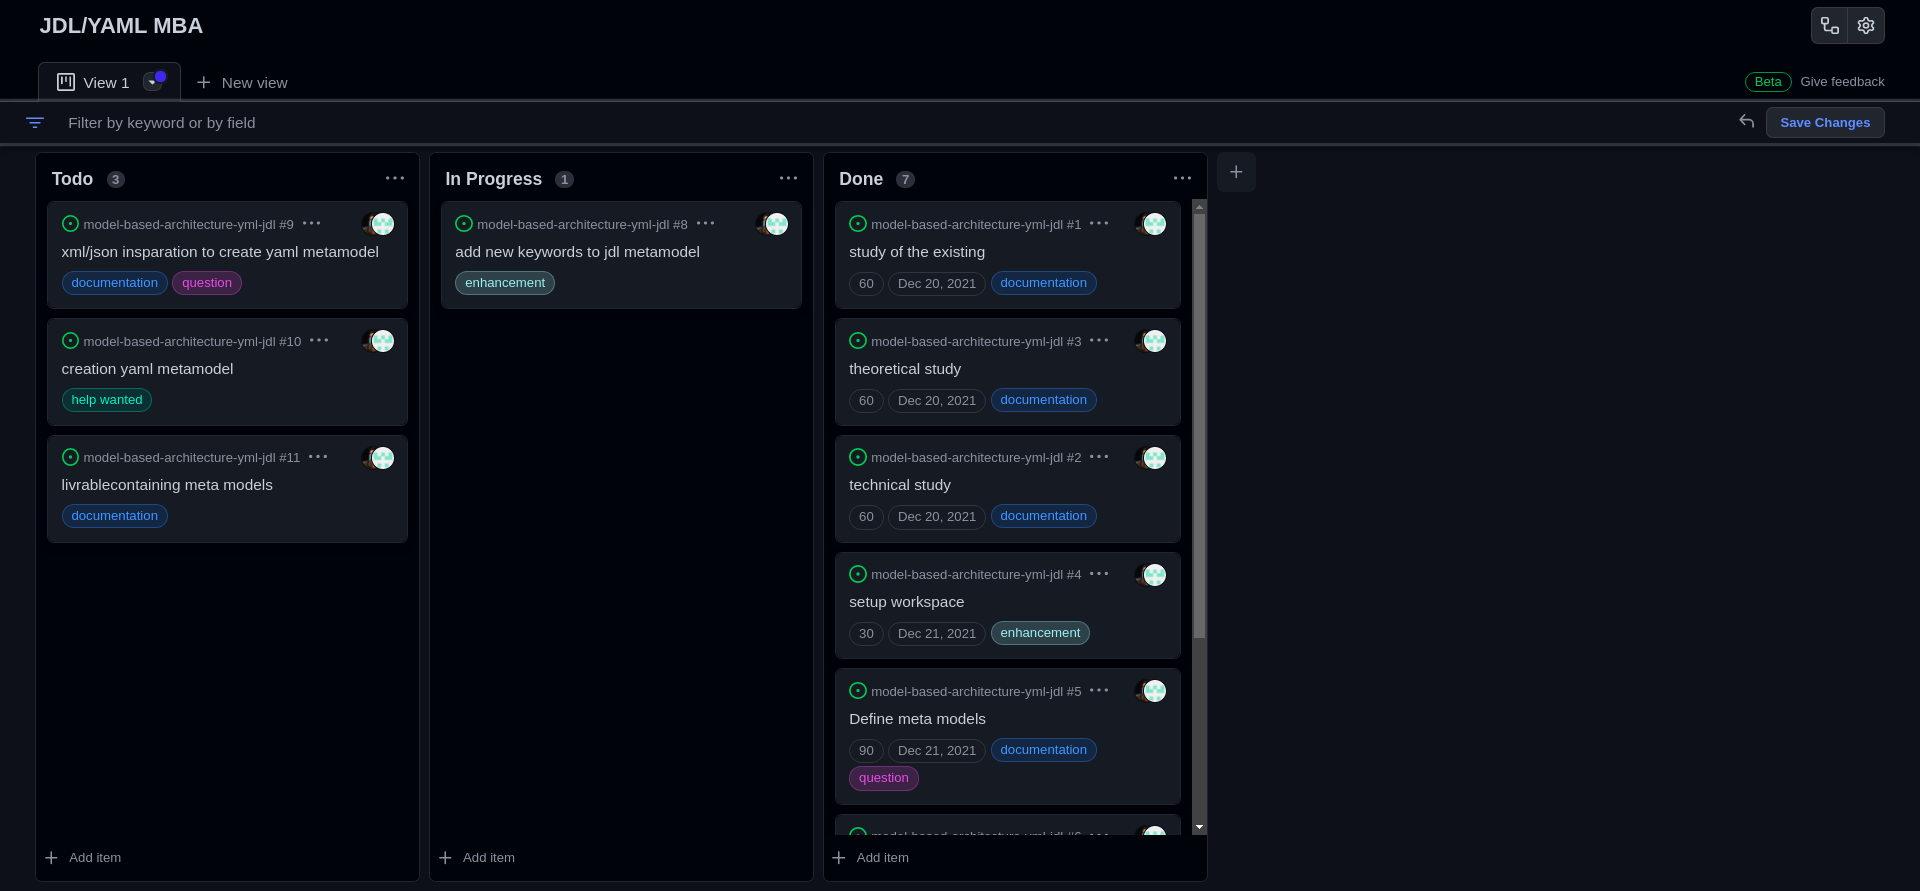
\includegraphics[width=16cm]{mode-trello.png}
      }
      \caption{Tableau Kanban pour la gestion des tâches}
  \end{center}
\end{figure}

Le modèle de tableau peut être représenté aussi sous-forme d'un tableau
contenant les mêmes informations d'une manières plus facile à
parcourir:

\begin{figure}[H]
  \begin{center}
      \fbox{
      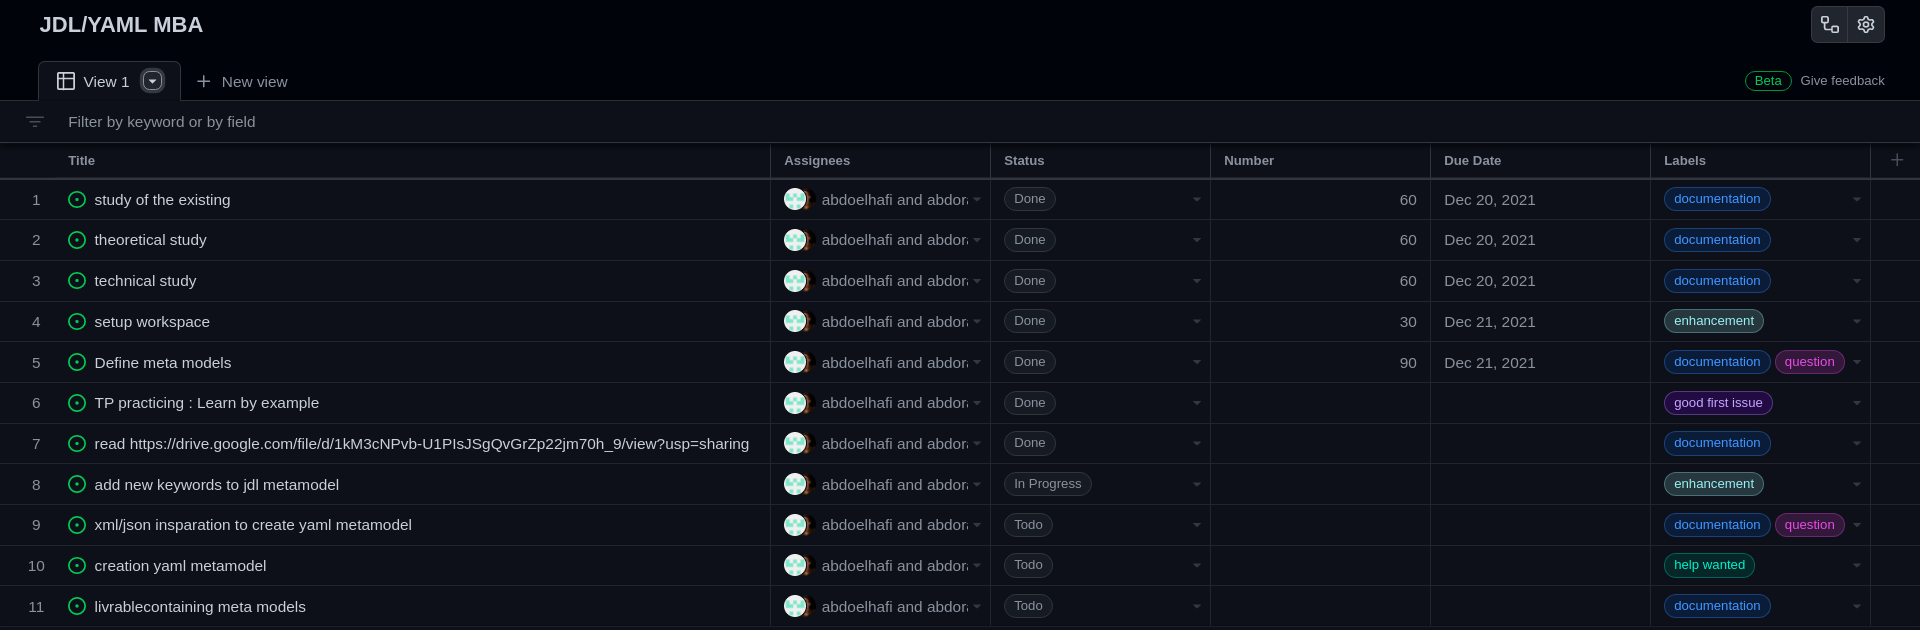
\includegraphics[width=16cm]{mode-table.png}
      }
      \caption{Tableau d'historiques des tâches}
  \end{center}
\end{figure}

Le cycle de vie d'un ticket dépend complétement de l'issue qu'en
concerne. Il se crée, prendre les dernières modification du issue, et
se label comme terminer si le issue est cloturé:

\begin{figure}[H]
  \begin{center}
      \fbox{
      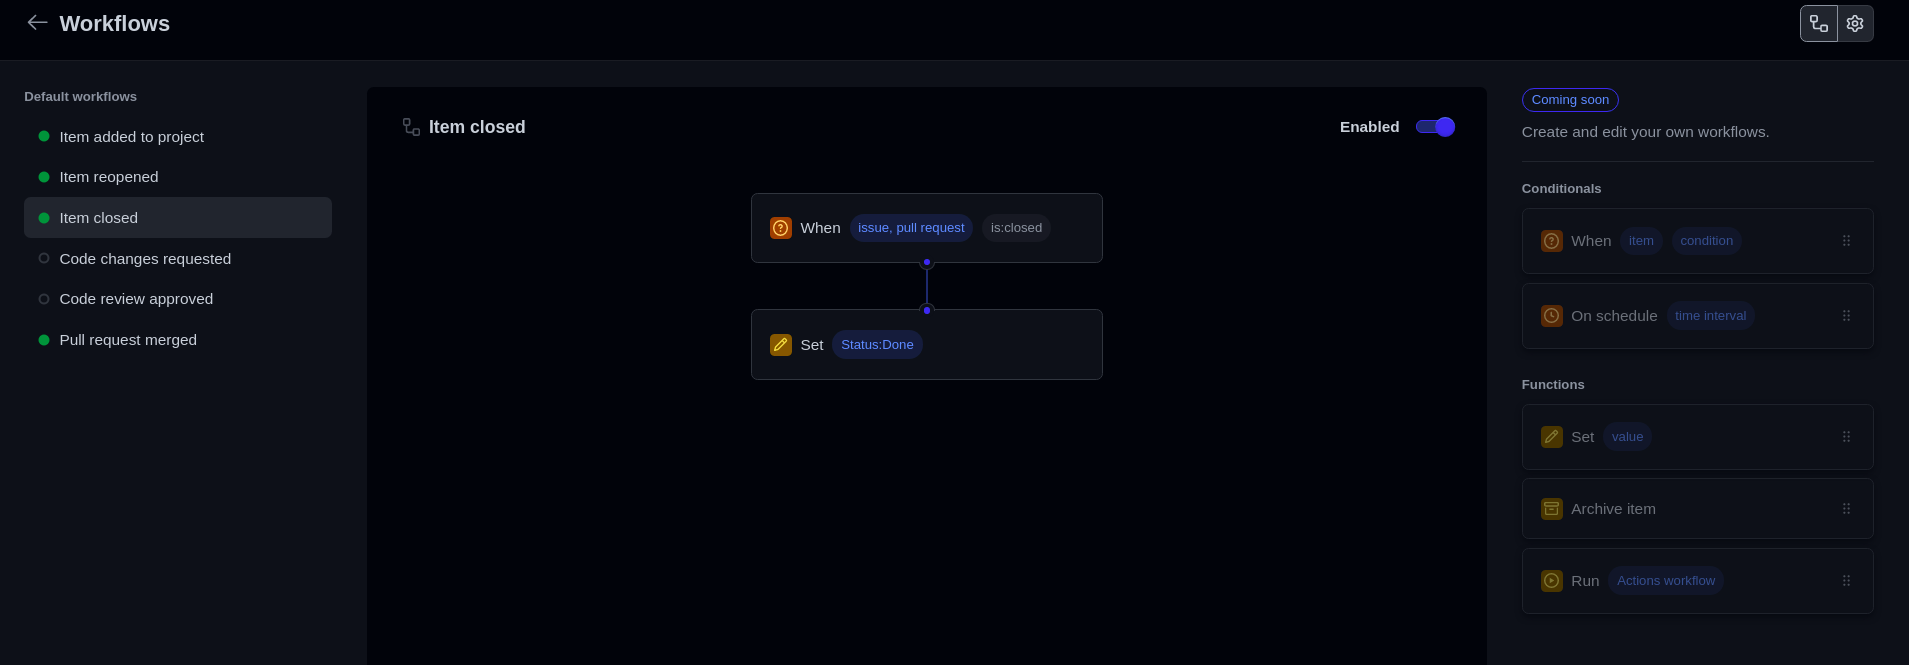
\includegraphics[width=16cm]{mode-automation.png}
      }
      \caption{Processus d'automation de la transformation des tâches en issues}
  \end{center}
\end{figure}

\section{Structure du projet}

La téchnologie utilisée dans ce projet est EMF. qui représente un
ensemble des outils trés puissants pour le MDSE. Ainsi, le projet a la structure suivante:

\begin{figure}[H]
  \begin{center}
      \fbox{
      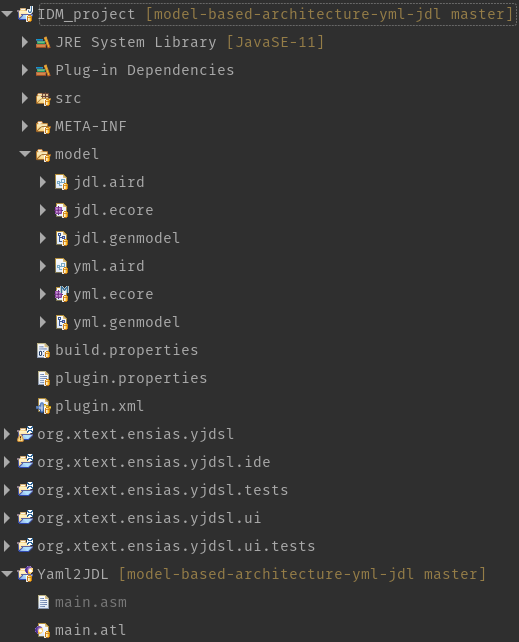
\includegraphics[width=16cm]{project structure.png}
      }
      \caption{Structure gloabale du projet}
  \end{center}
\end{figure}
